\documentclass[12pt,b5paper,openright,twoside]{book}
\usepackage{blindtext}
\usepackage{microtype}
\usepackage{listings}
\usepackage{color}
\usepackage{enumerate}
\usepackage{caption}
\usepackage{amsmath}
\usepackage{float}
\usepackage{algorithm}% http://ctan.org/pkg/algorithm
\usepackage{algpseudocode}% http://ctan.org/pkg/algorithmicx
\usepackage{graphicx}

\usepackage[utf8]{inputenc}
\usepackage[english]{babel}
\setlength{\parindent}{4em}
\setlength{\parskip}{1em}
%\usepackage{geometry}
%\geometry{
% b5paper
% }
\setcounter{chapter}{12}
\renewcommand{\chaptername}{Bab} 
%\title{BAB 13}
%\author{muhammadwidyan36 }
%\date{January 2016}

%\usepackage{natbib}
\usepackage{graphicx}
\usepackage{hyperref}
\usepackage{lmodern}
\hypersetup{
    colorlinks=true,
    linkcolor=blue,
    filecolor=magenta,      
    urlcolor=cyan,
    pdftitle={Sharelatex Example},
    pdfpagemode=FullScreen,
    }
\definecolor{dkgreen}{rgb}{0,0.6,0}
\definecolor{gray}{rgb}{0.5,0.5,0.5}
\definecolor{mauve}{rgb}{0.58,0,0.82}
\lstset{frame=tb,
  language=Java,
  aboveskip=3mm,
  belowskip=3mm,
  showstringspaces=false,
  columns=flexible,
  basicstyle={\small\ttfamily},
  numbers=none,
  numberstyle=\small\ttfamily\color{black},
  keywordstyle=\color{blue},
  commentstyle=\color{dkgreen},
  stringstyle=\color{mauve},
  breaklines=true,
  breakatwhitespace=true,
  tabsize=3
}

\urlstyle{same}

\begin{document}

%\maketitle
\chapter{Arrays of Objects}
\section{Tujuan}

Dalam tiga bab selanjutnya kita akan mengembangkan beberapa program yang dapat bekerja dengan permainan kartu(\textit{cards}) dan tumpukan kartu(\textit{decks of card}). Sebelum mempelajari lebih dalam, terdapat point-point secara garis besar :
\begin{enumerate}
 \item Dalam bab ini kita akan mendefinisikan kelas Card dan menulis \textit{method} yang bekerja pada kelas Kartu(\textit{Card}) dan Array dari Kartu(\textit{Card}) tersebut.
  \item Dalam bab 14 kita akan membuat kelas Tumpukan(\textit{decks}) dan menulis \textit{method} yang beroperasi pada kelas Tumpukan(\textit{decks}).
  \item Dalam bab 15 saya akan menyajikan program berorientasi objek (OOP) dan kita akan mengubah kelas Kartu(\textit{Card}) dan Tumpukan(\textit{decks}) menjadi OOP.
\end{enumerate}

Saya pikir bahwa point diatas agar mudah memahami untuk mencapai tujuan kita; Kekurangannya adalah bahwa kita akan melihat beberapa versi dari kode yang sama, yang dapat membingungkan. Jika membantu, Anda dapat mengunduh kode untuk setiap bab agar Anda dapat mengikuti. Anda dapat melihat Kode program untuk bab ini, pada link di sini : \url{http://thinkapjava.com/code/Card1.java} .

\section{Card objects}
Jika Anda belum merasa terbiasa dengan bermain kartu, sekarang adalah saat yang tepat untuk mendapatkan tumpukan kartunya, atau lainnya. Mungkin bab ini sedikit tidak masuk akal. Atau Anda dapat membaca lebih dahulu \url{http://en.wikipedia.org/wiki/Playing_card} .
Terdapat 52 lembar kartu dalam tumpukan yang terbagi menjadi empat jenis kartu, masing-masing terdiri 13 kartu. Jenis pasangan kartu itu adalah Sekop, Hati, Berlian dan Pohon. Urutan dalam kartu itu adalah As, 2, 3, 4, 5, 6, 7, 8, 9, 10, \textit{Jack}, \textit{Queen} dan \textit{King}. Tergantung pada apa permainan Anda bermain, \textit{As} dapat dianggap lebih tinggi dari \textit{King} atau lebih rendah dari 2. \par

\noindent Jika kita ingin mendefinisikan objek baru untuk bermain kartu, itu cukup jelas variabel apa yang misalnya harus: pangkat(\textit{ranks}) dan jenis pasangannya(\textit{suits}). Hal ini tidak jelas, jenis variabel apa yang harus digunakan. Salah satu kemungkinan adalah \textit{Strings}, yang berisikan seperti "Sekop" untuk jenisnya(\textit{suits}) dan "Queen" untuk pangkat(\textit{ranks}). Satu masalah dengan implementasi ini adalah bahwa hal itu tidak akan mudah untuk membandingkan kartu untuk melihat mana yang memiliki peringkat yang lebih tinggi atau jenis pasangannya.

\noindent Langkah alternatifnya adalah dengan menggunakan bilangan bulat untuk mengkodekan pangkat(\textit{ranks}) dan jenis pasangannya({\textit{suits}}). Dengan "encode" Saya tidak bermaksud seperti apa yang orang pikir, yaitu untuk mengenkripsi atau diterjemahkan ke dalam kode unik. Seorang ilmuwan komputer mengartikan "encode" adalah sesuatu seperti "mendefinisikan pemetaan antara urutan angka dan hal yang akan direpresentasikan." Misalnya :
\noindent 
\newline Sekop $\,\to\,$ 3 
\newline Hati $\,\to\,$ 2 
\newline Berlian  $\,\to\,$ 1 
\newline Pohon $\,\to\,$ 0 \par

\noindent Fitur yang jelas dari pemetaan ini adalah pemberian jenis pasangan(\textit{suits}) dengan bilangan bulat(\textit{integer}) dalam urutan, sehingga kita dapat membandingkan jenis pasangannya dengan membandingkan bilangan bulat(\textit{integer}). Pemetaan untuk pangkat(\textit{ranks}) cukup jelas; masing-masing pangkat numerik dipetakan ke bilangan yang sesuai, dan untuk tampilan kartu: 
\noindent 
\newline Jack $\,\to\,$ 11 
\newline Queen $\,\to\,$ 12 
\newline King  $\,\to\,$ 13 \par

\noindent Alasan saya menggunakan notasi matematika untuk pemetaan ini adalah bahwa mereka bukan bagian dari program. Mereka adalah bagian dari desain program, tetapi mereka tidak pernah muncul secara eksplisit dalam kode. Definisi kelas untuk Kartu(\textit{Cards}) terlihat seperti ini:

\begin{lstlisting}
class Card { 
    int suit, rank;
    public Card() { 
        this.suit = 0; this.rank = 0; 
    }
    public Card(int suit, int rank) { 
        this.suit = suit; this.rank = rank; 
    }
}

\end{lstlisting} \par 

\noindent Seperti biasa, saya menyediakan dua konstruktor: satu dengan parameter untuk setiap variabelnya. yang satunya tidak ada parameter.
\noindent 
\newline
\newline Untuk membuat objek yang mewakili 3 dari Pohon, kita membuat objek baru: 

\begin{lstlisting}
Card threeOfClubs = Card baru (0, 3); 
\end{lstlisting}

\noindent Argumen pertama, 0 mewakili jenis pasangan(\textit{suits}) Pohon.

\section{printCard method}
Bila Anda membuat kelas baru, langkah pertama adalah untuk menyatakan \textit{instance variabel} dan membuat konstruktor. Langkah kedua adalah untuk menulis \textit{standar method}, dimana harus memiliki setiap objek termasuk salah satu yang mencetak objek tersebut, dan satu atau dua yang membandingkan objek tersebut. Mari kita mulai dengan \textbf{printCard}.
 
\noindent Untuk mencetak objek Card dan dapat dibaca dengan mudah, kita ingin memetakan kode bilangan bulat(\textit{integer}) kedalam kata-kata. Cara untuk melakukannya adalah dengan array String. Anda dapat membuat array String dengan cara yang sama dengan Anda membuat sebuah array tipe primitif: 
\begin{lstlisting}
String [] suits = new String [4];
\end{lstlisting}

\noindent Maka kita dapat memberi nilai kedalam elemen array.
\begin{lstlisting}
suits [0] = "Pohon";
suits [1] = "Berlian";
suits [2] = "Hati";
suits [3] = "Sekop";
\end{lstlisting}

\noindent Membuat sebuah array dan menginisialisasi elemen adalah suatu operasi umum bahwa Java menyediakan sintaks khusus untuk itu:
\begin{lstlisting}
String[] suits = { "Pohon", "Berlian", "Hati", "Sekop" };
\end{lstlisting}

\noindent Pernyataan ini setara dengan deklarasi secara terpisah, alokasi, dan penugasan. Diagram array ini terlihat seperti:
\begin{figure}[h!]
\centering
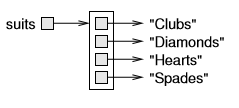
\includegraphics[scale=1]{diagram_array.png}
\caption{Ilustrasi Array}
\label{fig:univerise}
\end{figure}

\noindent Elemen-elemen dari array itu adalah referensi ke Strings, bukan Strings sendiri. Sekarang kita perlu array Strings lain untuk menginisialisasi pangkat(\textit{ranks}):
\begin{lstlisting}
String[] ranks = { "narf", "Ace", "2", "3", "4", "5", "6", "7", "8",    "9", "10", "Jack", "Queen", "King" };
\end{lstlisting}

\noindent Alasan terdapat element "narf" pada index nol adalah sebagai tempat untuk menjaga element pada index ke nol dari array, yang tidak pernah digunakan (atau seharusnya tidak digunakan). Satu-satunya pangkat yang valid adalah 1-13. Untuk menghindari elemen terbuang ini, kita bisa mulai pada 0, tetapi pemetaan yang lebih baik jika kita mengkodekan index array ke-2 sebagai 2, dan 3 sebagai 3, dll.
Menggunakan array ini, kita dapat memilih Strings yang sesuai dengan menggunakan pasangannya dan peringkat sebagai indeks. Dalam metode \textbf{printCard},
\begin{lstlisting}
public static void printCard(Card c) { 
    String[] suits = { "Pohon", "Berlian", "Hati", "Sekop" }; 
    String[] ranks = { "narf", "Ace", "2", "3", "4", "5", "6", "7", "8", "9", "10", "Jack", "Queen", "King" };
    System.out.println(ranks[c.rank] + " of " + suits[c.suit]);
}
\end{lstlisting}

\noindent fungsi [c.suit] berarti "menggunakan variabel suits dari objek c sebagai indeks ke dalam array bernama suits, dan pilih string yang sesuai." Output dari kode ini 
\begin{lstlisting}
Card card = new Card (1, 11); 
printCard (kartu);
\end{lstlisting}

\noindent adalah 
\begin{lstlisting} 
Jack of Berlian 
\end{lstlisting}

\section{sameCard method}
Kata "same" adalah salah satu dari banyak hal yang terjadi dalam sehari-hari yang tampak sangat jelas sampai Anda memberikan beberapa pemikiran, dan kemudian Anda menyadari ada yang lebih dari yang Anda harapkan.

\noindent Sebagai contoh, jika saya mengatakan "Chris dan saya memiliki mobil yang sama," Saya beranggapan bahwa mobilnya dan mobil saya adalah memiliki model yang sama dan cara pembuatan yang sama, tetapi mereka memiliki dua mobil yang berbeda. 

\noindent Jika saya mengatakan "Chris dan saya memiliki ibu yang sama," Saya beranggapan bahwa ibunya dan ibu saya adalah salah satu orang yang sama. Jadi gagasan "kesamaan" adalah berbeda tergantung pada konteks.

\noindent Ketika Anda berbicara tentang obyek, ada ambiguitas serupa. Sebagai contoh, jika dua kartu yang sama, apakah itu berarti mereka berisi data yang sama (pangkat dan pasangan/jenis), atau mereka benar-benar obyek Kartu yang sama?

\noindent Untuk melihat apakah dua referensi mengacu pada objek yang sama, kita menggunakan operator ==. Sebagai contoh:
\begin{lstlisting}
Card card1 = new Card(1, 11); 
Card card2 = card1;
if (card1 == card2) { 
    System.out.println("card1 and card2 are identical."); 
}
\end{lstlisting}

\noindent Referensi ke objek yang sama adalah identik. Referensi ke obyek dengan data yang sama adalah sama.
Untuk memeriksa kesetaraan, itu adalah umum untuk menulis sebuah \textit{method} dengan nama seperti \textbf{sameCard}.
\begin{lstlisting}
public static boolean sameCard(Card c1, Card c2) { 
    return(c1.suit == c2.suit && c1.rank == c2.rank); 
}
\end{lstlisting}

\noindent Berikut adalah contoh membuat dua objek dengan data yang sama, dan menggunakan \textbf{sameCard} untuk melihat apakah mereka adalah sama:
\begin{lstlisting}
Card card1 = new Card(1, 11); 
Card card2 = new Card(1, 11);
if (sameCard(card1, card2)) { 
    System.out.println("card1 and card2 are equivalent.");
}
\end{lstlisting}

\noindent Jika referensi identik, mereka juga setara, tetapi jika mereka setara, mereka tidak selalu identik.
Dalam hal ini, card1 dan card2 yang setara tetapi tidak identik, sehingga diagram array terlihat seperti ini:
\begin{figure}[h!]
\centering
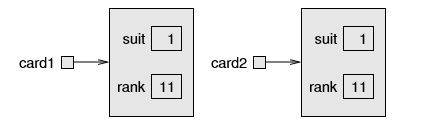
\includegraphics[scale=0.7]{diagram_array2.png}
\caption{Ilustrasi Array 2 objek}
\label{fig:univerise2}
\end{figure} \par

\noindent
\newline 
\newline 
\newline Apa yang terlihat seperti ketika card1 dan card2 identik?
Dalam Bagian 8.10 saya mengatakan bahwa Anda tidak harus menggunakan operator == pada Strings karena tidak melakukan apa yang Anda harapkan. Sebagai gantinya untuk membandingkan isi String (kesetaraan), ialah dengan mengecek apakah kedua String adalah objek yang sama (identitas).

\section{compareCard method}
Untuk tipe primitif, operator kondisional membandingkan nilai dan menentukan kapan yang satu lebih besar atau kurang dari yang lain. Operator ini (\textless  dan \textgreater dan lain-lain) tidak bekerja untuk jenis objek. Untuk String Java menyediakan \textit{method} \textbf{compareTo}. Untuk kelas Cards kita harus menulisnya sendiri, yang mana yang akan kita sebut \textbf{compareCard}. Kemudian, kita akan menggunakan \textit{method} ini untuk menyortir setumpuk(\textit{decks}) kartu.

\noindent Beberapa elemen memang terurut, yang berarti bahwa Anda dapat membandingkan dua elemen dan memberitahu mana yang lebih besar. Bilangan bulat dan bilangan desimal yang benar-benar menentukan. Beberapa tidak terurut, yang berarti bahwa tidak ada cara yang berarti untuk mengatakan bahwa salah satu element yang lebih besar dari yang lain. 

\noindent Buah-buahan termasuk kedalam tidak terurut, yang mengapa kita tidak bisa membandingkan antara apel dan jeruk. Di Java, jenis boolean adalah tidak terurut; kita tidak bisa mengatakan bahwa yang \textbf{true} adalah lebih besar dari yang \textbf{false}.

\noindent Element permainan kartu sebagian terurut, yang berarti bahwa kadang-kadang kita dapat membandingkan kartu dan kadang-kadang tidak. Sebagai contoh, saya tahu bahwa 3 Pohon lebih tinggi dari 2 Pohon, dan 3 Berlian lebih tinggi dari 3 Pohon. Tapi yang lebih baik, 3 Pohon atau 2 Berlian? Satu memiliki pangkat(\textit{ranks}) yang lebih tinggi, tetapi yang lain memiliki jenis pasangan(\textit{suits}) yang lebih tinggi.

\noindent Untuk membuat kartu sebanding, kita harus memutuskan mana yang lebih penting, pangkat(\textit{ranks}) atau jenis pasangan(\textit{suits}) kartu. Pilihannya adalah bebas, tetapi ketika Anda membeli tumpukan kartu baru,  diurutkan dimulai dengan semua Pohon bersama-sama, diikuti oleh semua Berlian, dan sebagainya. Jadi tentukanlah jenis pasangan(\textit{suits}) yang lebih penting.

\noindent Dengan diputuskannya itu, kita dapat menulis \textbf{compareCard}. Dibutuhkan dua Cards sebagai parameter dan mengembalikan nilai 1 jika kartu pertama menang, -1 jika kartu kedua menang, dan 0 jika mereka setara.

\noindent Pertama kita bandingkan suits: 
\begin{lstlisting}
if (c1.suit > c2.suit) return 1; 
if (c1.suit < c2.suit) return -1; 
\end{lstlisting}

\noindent Jika pernyataan tidak benar, suits harus sama, dan kami harus membandingkan ranks: 
\begin{lstlisting}
if (c1.rank > c2.rank) return 1; 
if (c1.rank < c2.rank) return -1; 
\end{lstlisting}

\section{Arrays of cards}
Sekarang kita telah melihat beberapa contoh dari komposisi (kemampuan untuk menggabungkan fitur bahasa dalam berbagai pengaturan). Salah satu contoh pertama yang kita lihat adalah menggunakan \textit{method}. Contoh lain adalah struktur bersarang: Anda dapat menempatkan \textit{if statement} dalam \textit{while loop}, atau dalam \textit{if statement}, dll

\noindent Setelah melihat pola ini, dan setelah belajar tentang array dan objek, Anda tidak perlu heran untuk mengetahui bahwa Anda dapat membuat array dari objek. Dan Anda dapat mendefinisikan objek dengan array sebagai variabel misalnya; Anda dapat membuat array yang berisi array;
Anda dapat mendefinisikan objek yang berisi objek-objek, dan sebagainya. Dalam dua bab berikutnya kita akan melihat contoh kombinasi ini menggunakan objek Card.

\noindent Ini merupakah contoh membuat sebuah array dari 52 kartu:
\begin{lstlisting}
Card[] cards = new Card[52];
\end{lstlisting}

\noindent Berikut adalah diagram array untuk objek ini:
\begin{figure}[h!]
\centering
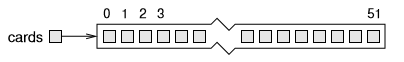
\includegraphics[scale=0.7]{diagram_array3.png}
\caption{Ilustrasi Array untuk objek}
\label{fig:univerise3}
\end{figure}

\noindent Array berisi referensi ke obyek; tidak mengandung objek Card sendiri. Unsur-unsur yang diinisialisasi ke null. Anda dapat mengakses elemen dari array dengan cara yang biasa:
\begin{lstlisting}
if (cards[0] == null) { 
    System.out.println("No cards yet!"); 
}
\end{lstlisting}
\noindent Tetapi jika Anda mencoba untuk mengakses variabel dari Cards yang tidak ada, Anda mendapatkan \textit{NullPointerException}.
\begin{lstlisting}
cards[0].rank;
\end{lstlisting}

\noindent Tapi itu adalah sintaks yang benar untuk mengakses rank dari "zeroeth" card dalam tumpukan kartu(\textit{decks}). Ini adalah contoh lain dari komposisi, menggabungkan sintaks untuk mengakses elemen array dan variabel instance dari objek.

\noindent Cara termudah untuk mengisi tumpukan dengan objek Card adalah menulis \textit{nested for} (yaitu, perulangan dalam perulangan) : 
\begin{lstlisting}
int index = 0; 
for (int suit = 0; suit <= 3; suit++) { 
    for (int rank = 1; rank <= 13; rank++) { 
        cards[index] = new Card(suit, rank); index++; 
    } 
}
\end{lstlisting}

\noindent Perulangan terluar menyebutkan setelan dari 0 sampai 3. Untuk masing-masing suits, perulangan didalam menyebutkan rank dari 1 sampai 13. Sejak perulangan terluar berjalan 4 kali, dan perulangan dalam menjalankan 13 kali, statement dalam perulangan itu dijalankan sebanyak 52 kali.

\noindent Saya menggunakan indeks untuk melacak di tumpukan mana kartu berikutnya harus keluar. Berikut diagram array menunjukkan tumpukan akan tampak seperti apa setelah kartu pertama dan kartu kedua telah dialokasikan:
\begin{figure}[h!]
\centering
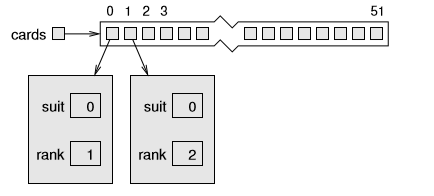
\includegraphics[scale=0.7]{array_in_for.png}
\caption{Ilustrasi Pengalokasian Array}
\label{fig:univerise4}
\end{figure}

\section{printDeck Method}
Ketika Anda bekerja dengan array, akan lebih mudah untuk memiliki \textit{method} yang mencetak isi dalam array tersebut. Kita telah melihat pola untuk melintasi array beberapa kali, sehingga \textit{method} berikut harus sudah biasa :
\begin{lstlisting}
public static void printDeck(Card[] cards) { 
    for (int i = 0; i < cards.length; i++) { 
        printCard(cards[i]); 
    } 
}
\end{lstlisting}

\noindent Sejak cards memiliki tipe data Card [], element cards memiliki tipe Card. Jadi cards [i] adalah argumen yang benar untuk \textbf{printCard}.

\section{Searching}
\textit{Method} berikutnya saya akan menulis adalah \textbf{findCard}, yang mencari array Cards untuk melihat apakah mengandung card tertentu. \textit{Method} ini memberi saya kesempatan untuk menunjukkan dua algoritma pencarian : \textbf{linear search} dan \textbf{bisection search}.

\noindent Pencarian linear cukup jelas; kita akan melintasi tumpukan(\textit{decks}) dan membandingkan setiap kartu dengan yang kita cari. Jika kita menemukan kartu itu kita mengembalikan indeks di mana kartu tersebut muncul. Jika tidak ditemukan, kita mengembalikan nilai -1.
\begin{lstlisting}
public static int findCard(Card[] cards, Card card) { 
    for (int i = 0; i< cards.length; i++) {
        if (sameCard(cards[i], card)) { 
            return i; 
        }
    } 
return -1;
}
\end{lstlisting}

\noindent Argumen \textbf{findCard} adalah card dan cards. Ini mungkin tampak aneh untuk memiliki sebuah variabel dengan nama yang sama sebagai jenis (variabel card memiliki tipe Card). Kita dapat membedakan karena variabel dimulai dengan huruf-huruf kecil. \textit{Method} akan mengembalikan nilai setelah menemukan card, yang berarti bahwa kita tidak harus melintasi seluruh tumpukan(\textit{decks}) kartu jika kita menemukan card yang kita cari. Jika kita sampai di akhir perulangan, kita tahu card tidak dalam tumpukan itu.

\noindent Jika card di dalam tumpukan tidak dalam urutan, tidak ada cara untuk mencari lebih cepat dari cara ini. Kita harus melihat setiap card karena kita tidak bisa memastikan card yang kita inginkan tidak ada. Tetapi ketika Anda mencari kata dalam kamus, Anda tidak menggunakan \textbf{linear search} melalui setiap kata, karena kata-kata dalam urutan abjad. Akibatnya, Anda mungkin menggunakan sebuah algoritma yang mirip dengan \textbf{bisection search}:
\begin{enumerate}
    \item Mulai di suatu tempat tengah.
    \item Pilih kata pada halaman dan membandingkannya dengan kata yang Anda cari.
    \item Jika Anda temukan kata yang Anda cari, berhenti.
    \item Jika kata yang Anda cari datang setelah kata pada halaman, balikan ke suatu tempat dan lanjutkan ke langkah 2.
    \item Jika kata yang Anda cari datang sebelum kata pada halaman, balikan ke suatu tempat sebelumnya dalam kamus dan lanjutkan ke langkah 2.
\end{enumerate}

\noindent Jika Anda pernah mendapatkan ke titik di mana ada dua kata yang berdekatan pada halaman dan kata-kata Anda berada diantara mereka, Anda dapat menyimpulkan bahwa kata-kata Anda tidak ada dalam kamus.
Kembali ke tumpukan card, jika kita tahu card dalam urutan, kita dapat menemukan lebih cepat dari \textbf{findCard}. Cara terbaik untuk menulis \textbf{bisection search} adalah dengan metode rekursif, karena \textit{bisection} secara alami rekursif.

\noindent Caranya adalah dengan menulis sebuah \textit{method} yang disebut \textbf{findBisect} yang mengambil dua indeks sebagai parameter, rendah dan tinggi, menunjukkan segmen dari array yang harus dicari (termasuk rendah dan tinggi).
\begin{enumerate}
    \item Untuk mencari array, memilih indeks antara rendah dan tinggi (menyebutnya pertengahan) dan bandingkan dengan kartu yang Anda cari.
    \item Jika Anda menemukannya, berhenti.
    \item Jika kartu di pertengahan lebih tinggi dari kartu Anda, cari kisaran dari rendah ke menengah 1.
    \item Jika kartu di pertengahan lebih rendah dari kartu Anda, cari kisaran dari pertengahan + 1 ke tinggi.
\end{enumerate}

\noindent Langkah 3 dan 4 terlihat seperti rekursif. 
Inilah apabila diterjemahkan ke dalam kode Java:

\begin{lstlisting}
public static int findBisect(Card[] cards, Card card, int low, int high) {
    // TODO: need a base case 
    int mid = (high + low) / 2; 
    int comp = compareCard(cards[mid], card);
    if (comp == 0) { 
        return mid; 
    } else if (comp > 0) { 
        return findBisect(cards, card, low, mid-1); 
    } else { 
        return findBisect(cards, card, mid+1, high); 
    }
}
\end{lstlisting}

\noindent Kode ini berisi kernel dari \textbf{bisection search}, tetapi masih hilang beberapa bagian penting, itulah sebabnya saya menambahkan komentar TODO. Seperti ditulis, \textit{method} recursif selamanya jika card tidak dalam tumpukan(\textit{decks}). Kita membutuhkan kasus dasar untuk menangani kondisi ini.
Jika tinggi memiliki nilai kurang dari rendah, tidak ada cards di antara mereka, kita simpulkan bahwa card tidak ada dalam tumpukan(\textit{decks}). Jika kita menangani kasus itu, \textit{method} ini bekerja dengan benar:
\begin{lstlisting}
public static int findBisect(Card[] cards, Card card, int low, int high) { 
    System.out.println(low + ", " + high);
    if (high < low) return -1;
        int mid = (high + low) / 2; int comp = compareCard(cards[mid], card);
    if (comp == 0) { 
        return mid;
    } else if (comp > 0) { 
        return findBisect(cards, card, low, mid-1); 
    } else { 
        return findBisect(cards, card, mid+1, high); 
    }
}
\end{lstlisting}

Saya menambahkan pernyataan \textit{print} sehingga saya bisa mengikuti urutan rekursif. Saya mencoba kode berikut: 
\begin{lstlisting}
Card  card1 = new Card (1, 11); 
System.out.println (findBisect (kartu, card1, 0, 51)); 
\end{lstlisting}

\noindent Dan mendapat output berikut: 
\newline 0, 51 
\newline 0, 24 
\newline 13, 24 
\newline 19, 24 
\newline 22, 24 
\newline 23 

\noindent Kemudian saya membuat card yang tidak berada dalam tumpukan (15 Berlian), dan mencoba untuk menemukannya. Saya mendapat hasil berikut: 
\newline 0, 51 
\newline 0, 24 
\newline 13, 24 
\newline 13, 17 
\newline 13, 14 
\newline 13, 12
\newline -1

\noindent Tes tersebut tidak membuktikan bahwa program ini benar. Bahkan, tidak ada jumlah pengujian dapat membuktikan bahwa program benar. Di sisi lain, dengan melihat beberapa kasus dan memeriksa kode, Anda mungkin bisa meyakinkan diri sendiri.
Jumlah rekursif biasanya 6 atau 7, jadi kita hanya memanggil \textbf{compareCard} 6 atau 7 kali, dibandingkan dengan hingga 52 kali jika kita melakukan \textbf{linear search}. Secara umum, \textit{bisection} jauh lebih cepat daripada \textbf{linear search}, dan bahkan lebih lagi dari pada array.
Dua kesalahan umum dalam program rekursif ialah melupakan untuk menyertakan kasus dasar dan menulis panggilan rekursif sehingga kasus dasar tidak pernah tercapai. 
Salah satu kesalahan menyebabkan rekursi yang tak hingga, yang akhirnya memunculkan \textit{StackOverflowException}. (Pikirkan diagram stack untuk metode rekursif yang tidak pernah berakhir.)

\section{Decks and subdecks}
Berikut adalah prototype dari \textbf{findBisect} :
\begin{lstlisting}
public static int findBisect(Card[] deck, Card card, int low, int high)
\end{lstlisting}

\noindent Kami bisa memikirkan kartu, rendah, dan tinggi sebagai parameter tunggal yang spesifik seperti subdeck . Cara berpikir umum, dan kadang-kadang disebut sebagai parameter abstrak. Yang saya maksud dengan "abstrak" adalah sesuatu yang tidak benar-benar bagian dari teks program, tapi yang menggambarkan fungsi program di tingkat yang lebih tinggi.

\noindent Sebagai contoh, ketika Anda memanggil \textit{method} dan melewati array dan batas-batasnya yang rendah dan tinggi, tidak ada yang mencegah untuk memanggil \textit{method} untuk mengakses bagian array yang di luar batas. Jadi Anda tidak benar-benar mengirimkan subset dari tumpukan tersebut; Anda benar-benar mengirimkan seluruh tumpukannya. Tapi selama penerima memainkan oleh aturan, masuk akal untuk berpikir tentang itu secara abstrak sebagai subdeck.

\noindent Pemikiran seperti ini, di mana program mengambil makna melampaui apa yang secara harfiah dikodekan, merupakan bagian penting dari berpikir seperti seorang ilmuwan komputer. Kata "abstrak" akan digunakan begitu sering dalam banyak konteks yang maknanya datang dan pergi begitu saja. Namun demikian, abstraksi adalah ide sentral dalam ilmu komputer (dan banyak bidang lain).

\noindent Yang lebih umum definisi dari "abstraksi" adalah "Proses pemodelan sistem yang kompleks dengan deskripsi sederhana untuk menyingkatkan rincian yang tidak perlu saat kita memahami perilaku yang relevan."

\section{Glossary}
\textbf{encode}: Untuk menyatakan satu set nilai-nilai dengan menggunakan satu set nilai-nilai lainnya, dengan membangun pemetaan diantara mereka.
\textbf{identity}: Kesetaraan referensi. Dua referensi yang mengarah ke objek yang sama di memori.
\textbf{equivalence}: Kesetaraan nilai. Dua referensi yang mengarah ke objek yang berisi data yang sama.
\textbf{abstract parameter}: Satu set parameter yang bertindak bersama-sama sebagai parameter tunggal.
\textbf{abstraction}: Proses menafsirkan program (atau apa pun) di tingkat yang lebih tinggi dari apa yang benar-benar diwakili oleh kode.

\section{Exercise}
Latihan 13.1. Merangkum kode dalam Bagian 13.5 dalam sebuah method. Kemudian memodifikasinya sehingga aces memiliki peringkat lebih tinggi dari Kings.

\noindent Latihan 13.2. Merangkum kode \textit{deck-building} Bagian 13.6 di \textit{method} yang disebut \textbf{makeDeck} yang tidak mempunyai parameter dan mengembalikan sebuah array dari Cards.

\noindent Latihan 13.3. Dalam Blackjack objek dari permainan ini adalah untuk mendapatkan koleksi kartu dengan skor 21. Skor yang berada di tangan adalah jumlah skor untuk semua kartu. Skor untuk As adalah 1, untuk semua kartu sepuluh, dan untuk semua kartu lain memiliki skor sama seperti pada \textit{ranks}. Contoh: di tangan (As, 10, Jack, 3) memiliki skor total 10 + 1 + 10 + 3 = 24.
Tulis sebuah \textit{method} yang disebut \textbf{handScore} yang mengambil array cards sebagai argumen dan yang mengembalikan skor total.

\noindent Latihan 13.4. Dalam poker sebuah "flush" adalah memiliki kartu yang berisi lima atau lebih kartu dari jenis yang sama. Dapat berisi banyak nomor dari kartu tersebut
\begin{enumerate}
    \item Tulis \textit{method} yang disebut \textbf{suitHist} yang mengambil array Cards sebagai parameter dan yang mengembalikan histogram dari jenis kartu yang berada di tangan. Solusi Anda hanya harus melintasi array sekali.
    \item Tulis \textit{method} yang disebut \textbf{hasFlush} yang mengambil array Cards sebagai parameter dan yang mengembalikan \textbf{true} jika berisi flush, dan \textbf{false} jika tidak.
\end{enumerate}

\noindent Latihan 13.5. Bekerja dengan kartu lebih menarik jika Anda dapat menampilkannya di layar. Jika Anda tidak bermain dengan contoh grafis, Anda mungkin ingin melakukan itu sekarang.
Pertama download \url{http://thinkapjava.com/code/CardTable.java} dan \url{http://thinkapjava.com/code/cardset.zip} simpan ke folder yang sama. Kemudian unzip cardset.zip, yang berisi subfolder cardset-oxymoron dengan semua gambar kartu. (Perhatikan cardset variabel di CardTable.main adalah nama folder ini.) Jalankan CardTable.java dan Anda akan melihat gambar dari pak kartu yang diletakkan di atas meja hijau.
Anda dapat menggunakan kelas ini sebagai tempat awal untuk menerapkan permainan kartu Anda sendiri

\end{document}
